\chapter{Conceptual Design}
Following the clarification of the task is the conceptual design, where in this section of the product development process, designers engage in creative exploration and evaluation of various design ideas and concepts.

According to Pahl and Beitz, conceptual design is the stage of the design process where important issues are pinpointed through abstraction  \cite[159]{Pahl2007}. The process involves establishing function structures, searching for suitable working principles, and ultimately combining these elements to create a working structure.

Figure \ref{fig:steps-conceptual-design} shows the steps involved in this phase.

\begin{figure}[ht!]
    \centering
    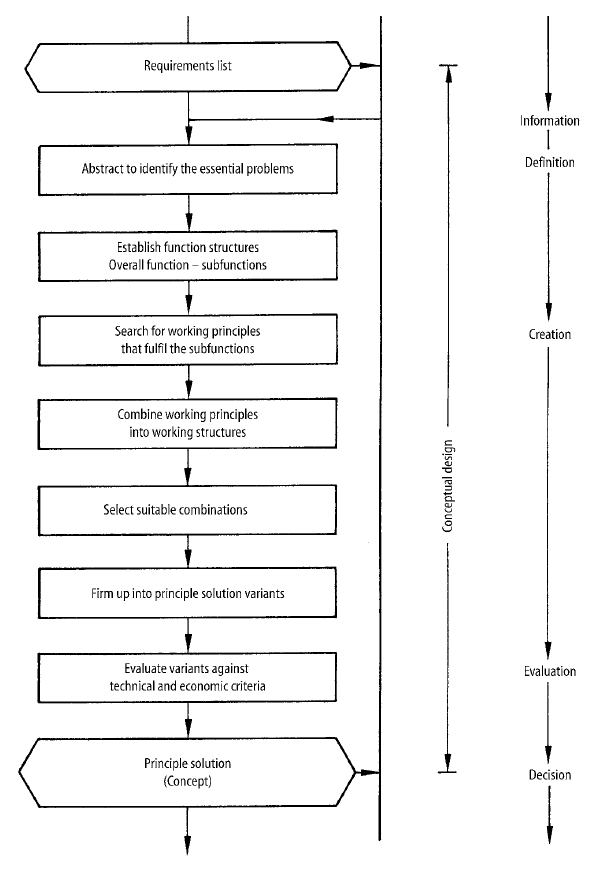
\includegraphics[width=0.7\linewidth]{texs/Part1/chapter3/image/conceptual.png}
    \caption{Steps in Conceptual Design \cite[160]{Pahl2007}}
    \label{fig:steps-conceptual-design}
\end{figure}


\section{Abstraction}
Due to new technologies, procedures, materials, and scientific discoveries, traditional solution principles or designs may not be able to provide optimal answers, and to overcome fixation on conventional ideas, designers utilize abstraction, focusing on the general and essential aspects rather than particular details \cite[161]{Pahl2007}.

To help in identification of the essential problems, following abstraction techniques are used \cite[165]{Pahl2007}:

\begin{itemize}
    \item \textbf{Step 1:} Eliminate personal preferences.
    \item \textbf{Step 2:} Omit requirements that have no direct bearing on the function and the essential constraints.
    \item \textbf{Step 3:} Transform quantitative into qualitative data and reduce them to essential statements.
    \item \textbf{Step 4:} Generalise the previous step's results.
    \item \textbf{Step 5:} Formulate the problem in solution-neutral terms.
\end{itemize}

Figure \ref{fig:result-abstraction-process} shows the result of the abstraction process.

\begin{figure}[ht!]
    \centering
    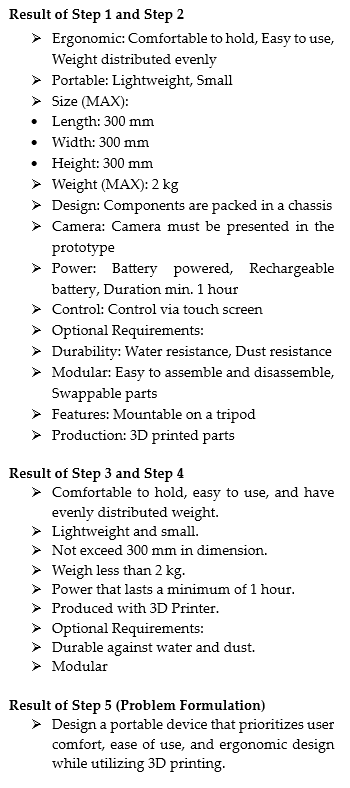
\includegraphics[width=0.4\linewidth]{texs/Part1/chapter3/image/abstractionresult.png}
    \caption{Result of Abstraction Process}
    \label{fig:result-abstraction-process}
\end{figure}


\section{Function Structures}
Pahl and Beitz \cite[31]{Pahl2007} define function structures as a graphical representation of the functions of a system and their interrelationships. It is a hierarchical representation of the functions of a system, starting with the overall function and breaking it down into sub-functions. The function structure is a helpful tool for identifying a system's essential functions and the relationships between the functions.

Figure \ref{fig:subfunction-break} shows the representation of the function structure and the process of breaking down the overall function into sub-functions.

\begin{figure}[ht!]
    \centering
    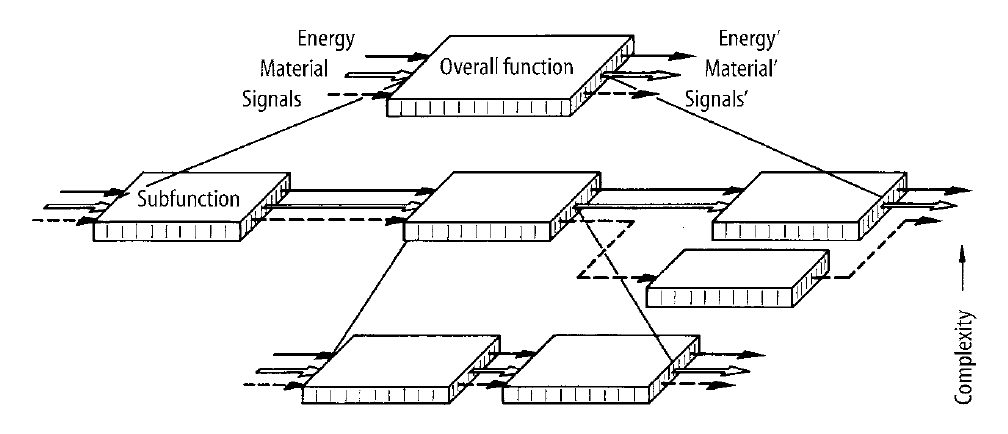
\includegraphics[width=0.8\linewidth]{texs/Part1/chapter3/image/subfunctionbreak.png}
    \caption{Breaking down the overall function into sub-functions \cite[32]{Pahl2007}}
    \label{fig:subfunction-break}
\end{figure}


\subsection{Overall Function}
Based on the result of abstraction, the system's overall function can be represented and visualized using a function structure diagram, as shown in Figure \ref{fig:overall-function}.

In this overall function, the prototype's components are defined as an input, while the prototype itself is defined as the output. The overall function is decomposed into sub-functions in the next section.

\begin{figure}[ht!]
    \centering
    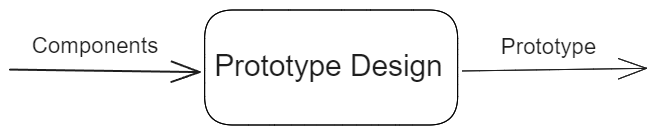
\includegraphics[width=0.5\linewidth]{texs/Part1/chapter3/image/overallfunction.png}
    \caption{Overall Function of the System}
    \label{fig:overall-function}
\end{figure}


\subsection{Sub-Functions}
\begin{figure}[ht!]
    \centering
    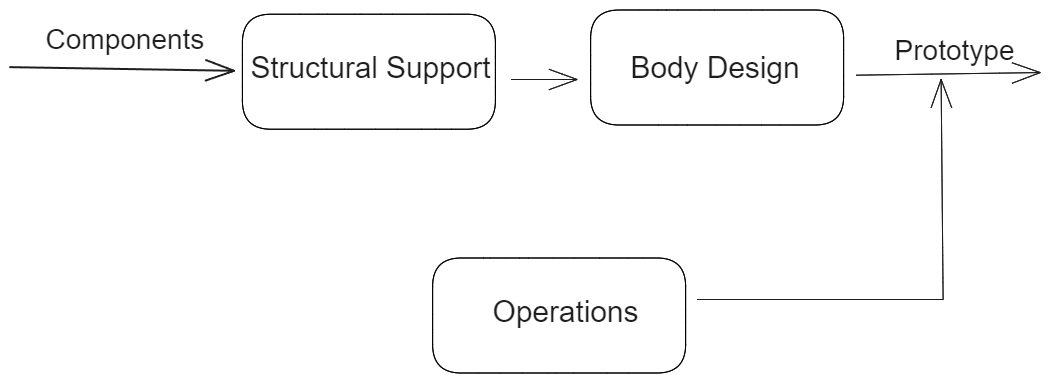
\includegraphics[width=0.8\linewidth]{texs/Part1/chapter3/image/subfunction1.png}
    \caption{Sub-Functions of the System}
    \label{fig:sub-functions}
\end{figure}

\begin{figure}[ht!]
    \centering
    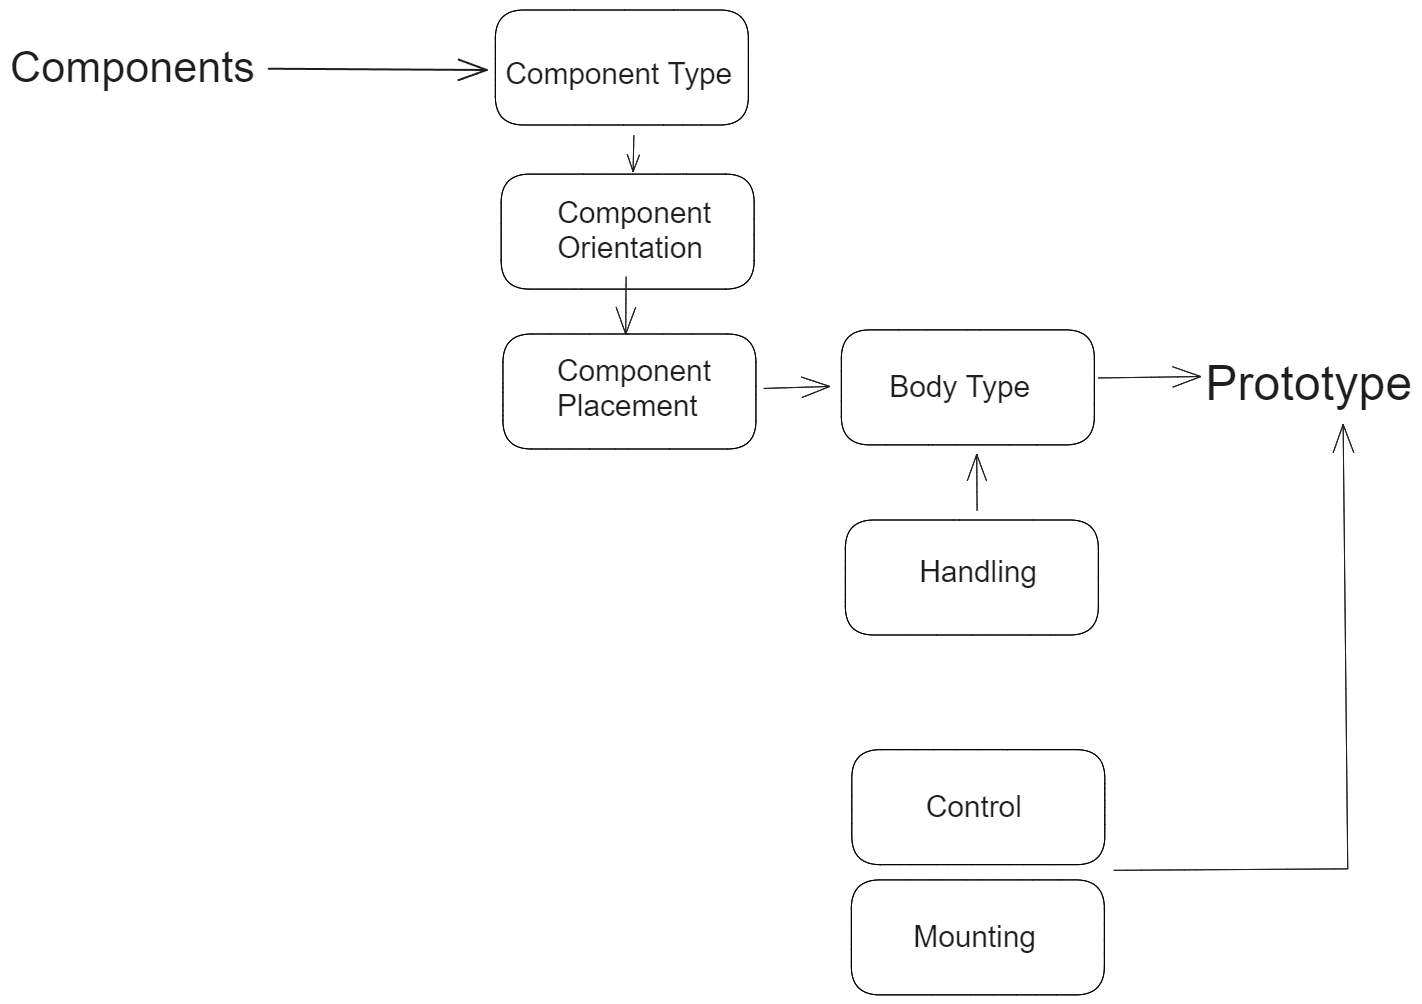
\includegraphics[width=\linewidth]{texs/Part1/chapter3/image/subfunction2.png}
    \caption{Sub-Functions of the System (Final)}
    \label{fig:sub-functions-final}
\end{figure}

Decomposing the overall function into sub-functions is crucial in the conceptual design process, and as described by Pahl and Beitz \cite[170]{Pahl2007}, the purpose of this decomposition is to reduce the complexity of the overall system and facilitate the identification of suitable solution principles that can fulfill the required functions.

Figure \ref{fig:sub-functions} illustrates the sub-functions of the prototype. Deriving from the overall function, labeled as \textit{Prototype Design}, it breaks down into three subfunctions, specifically \textit{Structural Support}, \textit{Body Design}, and \textit{Operation}. The function is then further decomposed into more detailed sub-functions in Figure \ref{fig:sub-functions-final}.

The term \textit{Structural Support} refers to the measures taken to ensure the structural integrity of the prototype. This sub-function encompasses activities such as securing and stabilizing the internal components within the prototype. To simplify the function, it decomposed into three sub-functions:  \textit{Component Placement}, which specifies the positioning of internal components; \textit{Component Orientation}, which details the alignment of internal components; and \textit{Component Type}, which is the type of component itself.

\textit{Body Design} describe the sub-functions involving the prototype's physical structure. To further simplify the task, this sub-function is decomposed into \textit{Body Type}, which defines the outline of the structure, and \textit{Handling}, which describes the handling of the prototype.

\textit{Operation} deals with how the prototype works. It describes the device's usage and the components involved during operation. This function is then divided into \textit{Control}, which describes the component involved into controlling input from user during operation, and \textit{Mounting}, which refers to the integration of the prototype with the tripod stand.

\section{Developing Working Principles}

As defined by Pahl and Beitz, working principles refer to the physical effects and characteristics that fulfill specific functions of the designed structure \cite[181]{Pahl2007}. These principles are combined to create the working structure, encompassing physical processes and the form design features. Several potential working structures can be generated by varying the physical effects and form design features, known as the solution field.

In developing working principles, there are multiple available methods in idea generation. These methods are categorized into three groups:

\begin{itemize}
    \item Conventional methods
    \item Intuitive methods
    \item Discursive methods
\end{itemize}

Pahl and Beitz \cite[18-82]{Pahl2007} describe the \textit{Conventional Methods} as a systematic and data-driven approach. Designers gather information from various sources, such as literature, trade publications, and competitor catalogs, to stay informed about advancements and best practices. They analyze natural systems and existing technical systems to draw inspiration and identify opportunities for improvement.

On the other hand, the \textit{Intuitive Methods}, as described by them \cite[82-89]{Pahl2007}, tap into creativity and associative thinking. \textit{Brainstorming} fosters a collaborative environment where diverse perspectives generate a wide range of ideas without judgment. \textit{Method 635} adds structure to Brainstorming, allowing for systematic idea development within a group. The \textit{Gallery Method} combines individual work with group discussions, using sketches or drawings to explore solution proposals visually.

Additionally, the \textit{Discursive methods} \cite[89-103]{Pahl2007} combines systematic, step-by-step procedures with elements of intuition and creativity. They involve deliberate analysis of physical processes, leading to multiple solution variants derived from the relationships between variables. This approach fosters a deeper understanding of the problem space.

\subsection{Searching for Working Principles}
\textit{Brainstorming} and \textit{Analysis of Existing Technical Systems} are utilized in this work to establish working principles. Table \ref{tab:classification-scheme-working-principles} shows the result of idea generation. For more detailed sketches of the working principles, please refer to Appendix \ref{appendix:sketches-of-working-principles}.

\begin{table}[H]
    \centering
    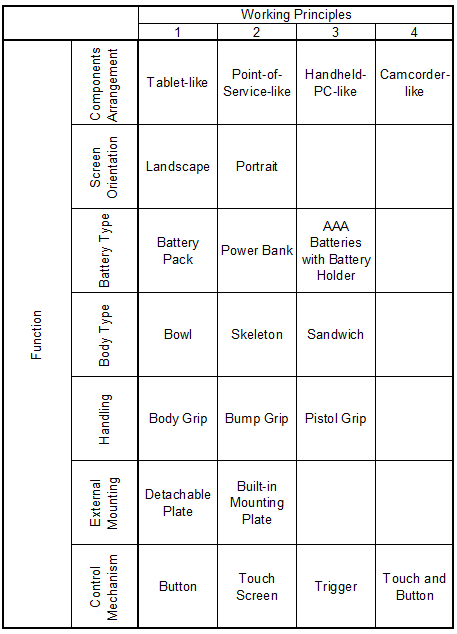
\includegraphics[width=0.6\linewidth]{texs/Part1/chapter3/image/stotal.png}
    \caption{Classification Scheme for Working Principles}
    \label{tab:classification-scheme-working-principles}
\end{table}


\section{Combination of Working Principles}
In this step, we will combine the working principles assigned to the sub-functions to create potential working structures. To achieve this, the identified working principles must be linked following the functional structure to fulfill the overall function.

The method we will employ for systematic combination is Zwicky's morphological box \cite{Kushahrin22}. In this approach, the potential principles are represented in a table for better clarity and connected to form functional structures using connecting lines.

Figure \ref{fig:morphological-chart-with-solution-variants} shows the morphological chart with the generated solution variants. The solution variants are labeled S1 to S8, with each color representing a different solution variant.

\begin{figure}[ht!]
    \centering
    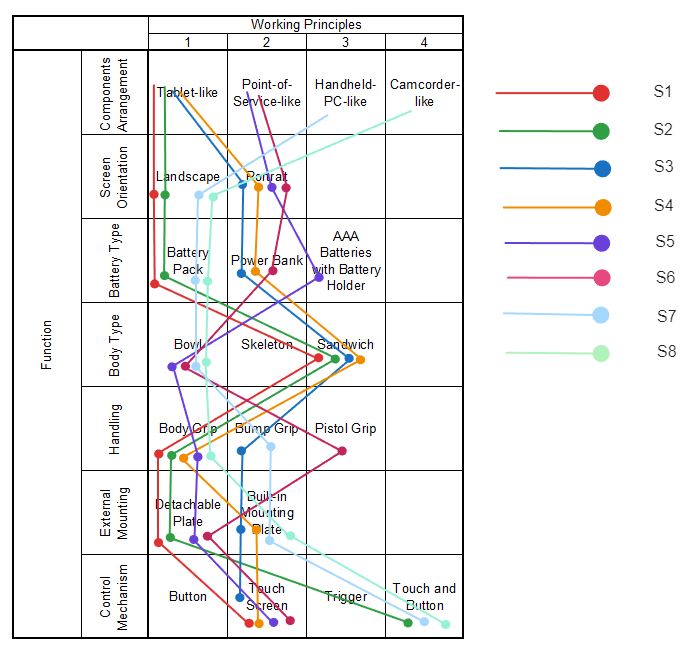
\includegraphics[width=\linewidth]{texs/Part1/chapter3/image/combinedchart.png}
    \caption{Morphological Chart with Solution Variants}
    \label{fig:morphological-chart-with-solution-variants}
\end{figure}

\section{Firming Up into Principle Solution Variants}
In this section, we showcase hand-drawn sketches of identified functional structures that have been transformed into practical solution alternatives. Each sketch is accompanied by a brief description of its operations, highlighting its potential strengths and weaknesses. The sketches are based on the result of the morphological chart in Figure \ref{fig:morphological-chart-with-solution-variants}.

\subsection{Solution Variant 1, S1}
In Solution Variant 1, we encounter a tablet-like design that closely resembles a typical tablet device. The key components, including the Raspberry Pi, Battery, Camera, and Screen, are arranged in a manner similar to a tablet. The screen orientation is in landscape mode, offering a broader display view for enhanced visual clarity. This orientation is particularly beneficial when the device is used for tasks that require a wider viewing area.

The design is thoughtfully optimized for handheld use, featuring a body grip that ensures comfortable handling. The internal battery integration contributes to a seamless and integrated appearance. A sandwich-type body provides robust protection for the internal components, comprising a top cover, main body, and bottom cover.

For mounting purposes, Solution Variant 1 utilizes a detachable plate tripod system, offering the convenience of easy attachment and removal from a tripod stand. The primary control mechanism for this variant is a touch screen, allowing for intuitive and user-friendly interactions with the device's functionalities.

Figure \ref{fig:sketch-solution-variant-1} shows the sketch of Solution Variant 1.

\begin{figure}[H]
    \centering
    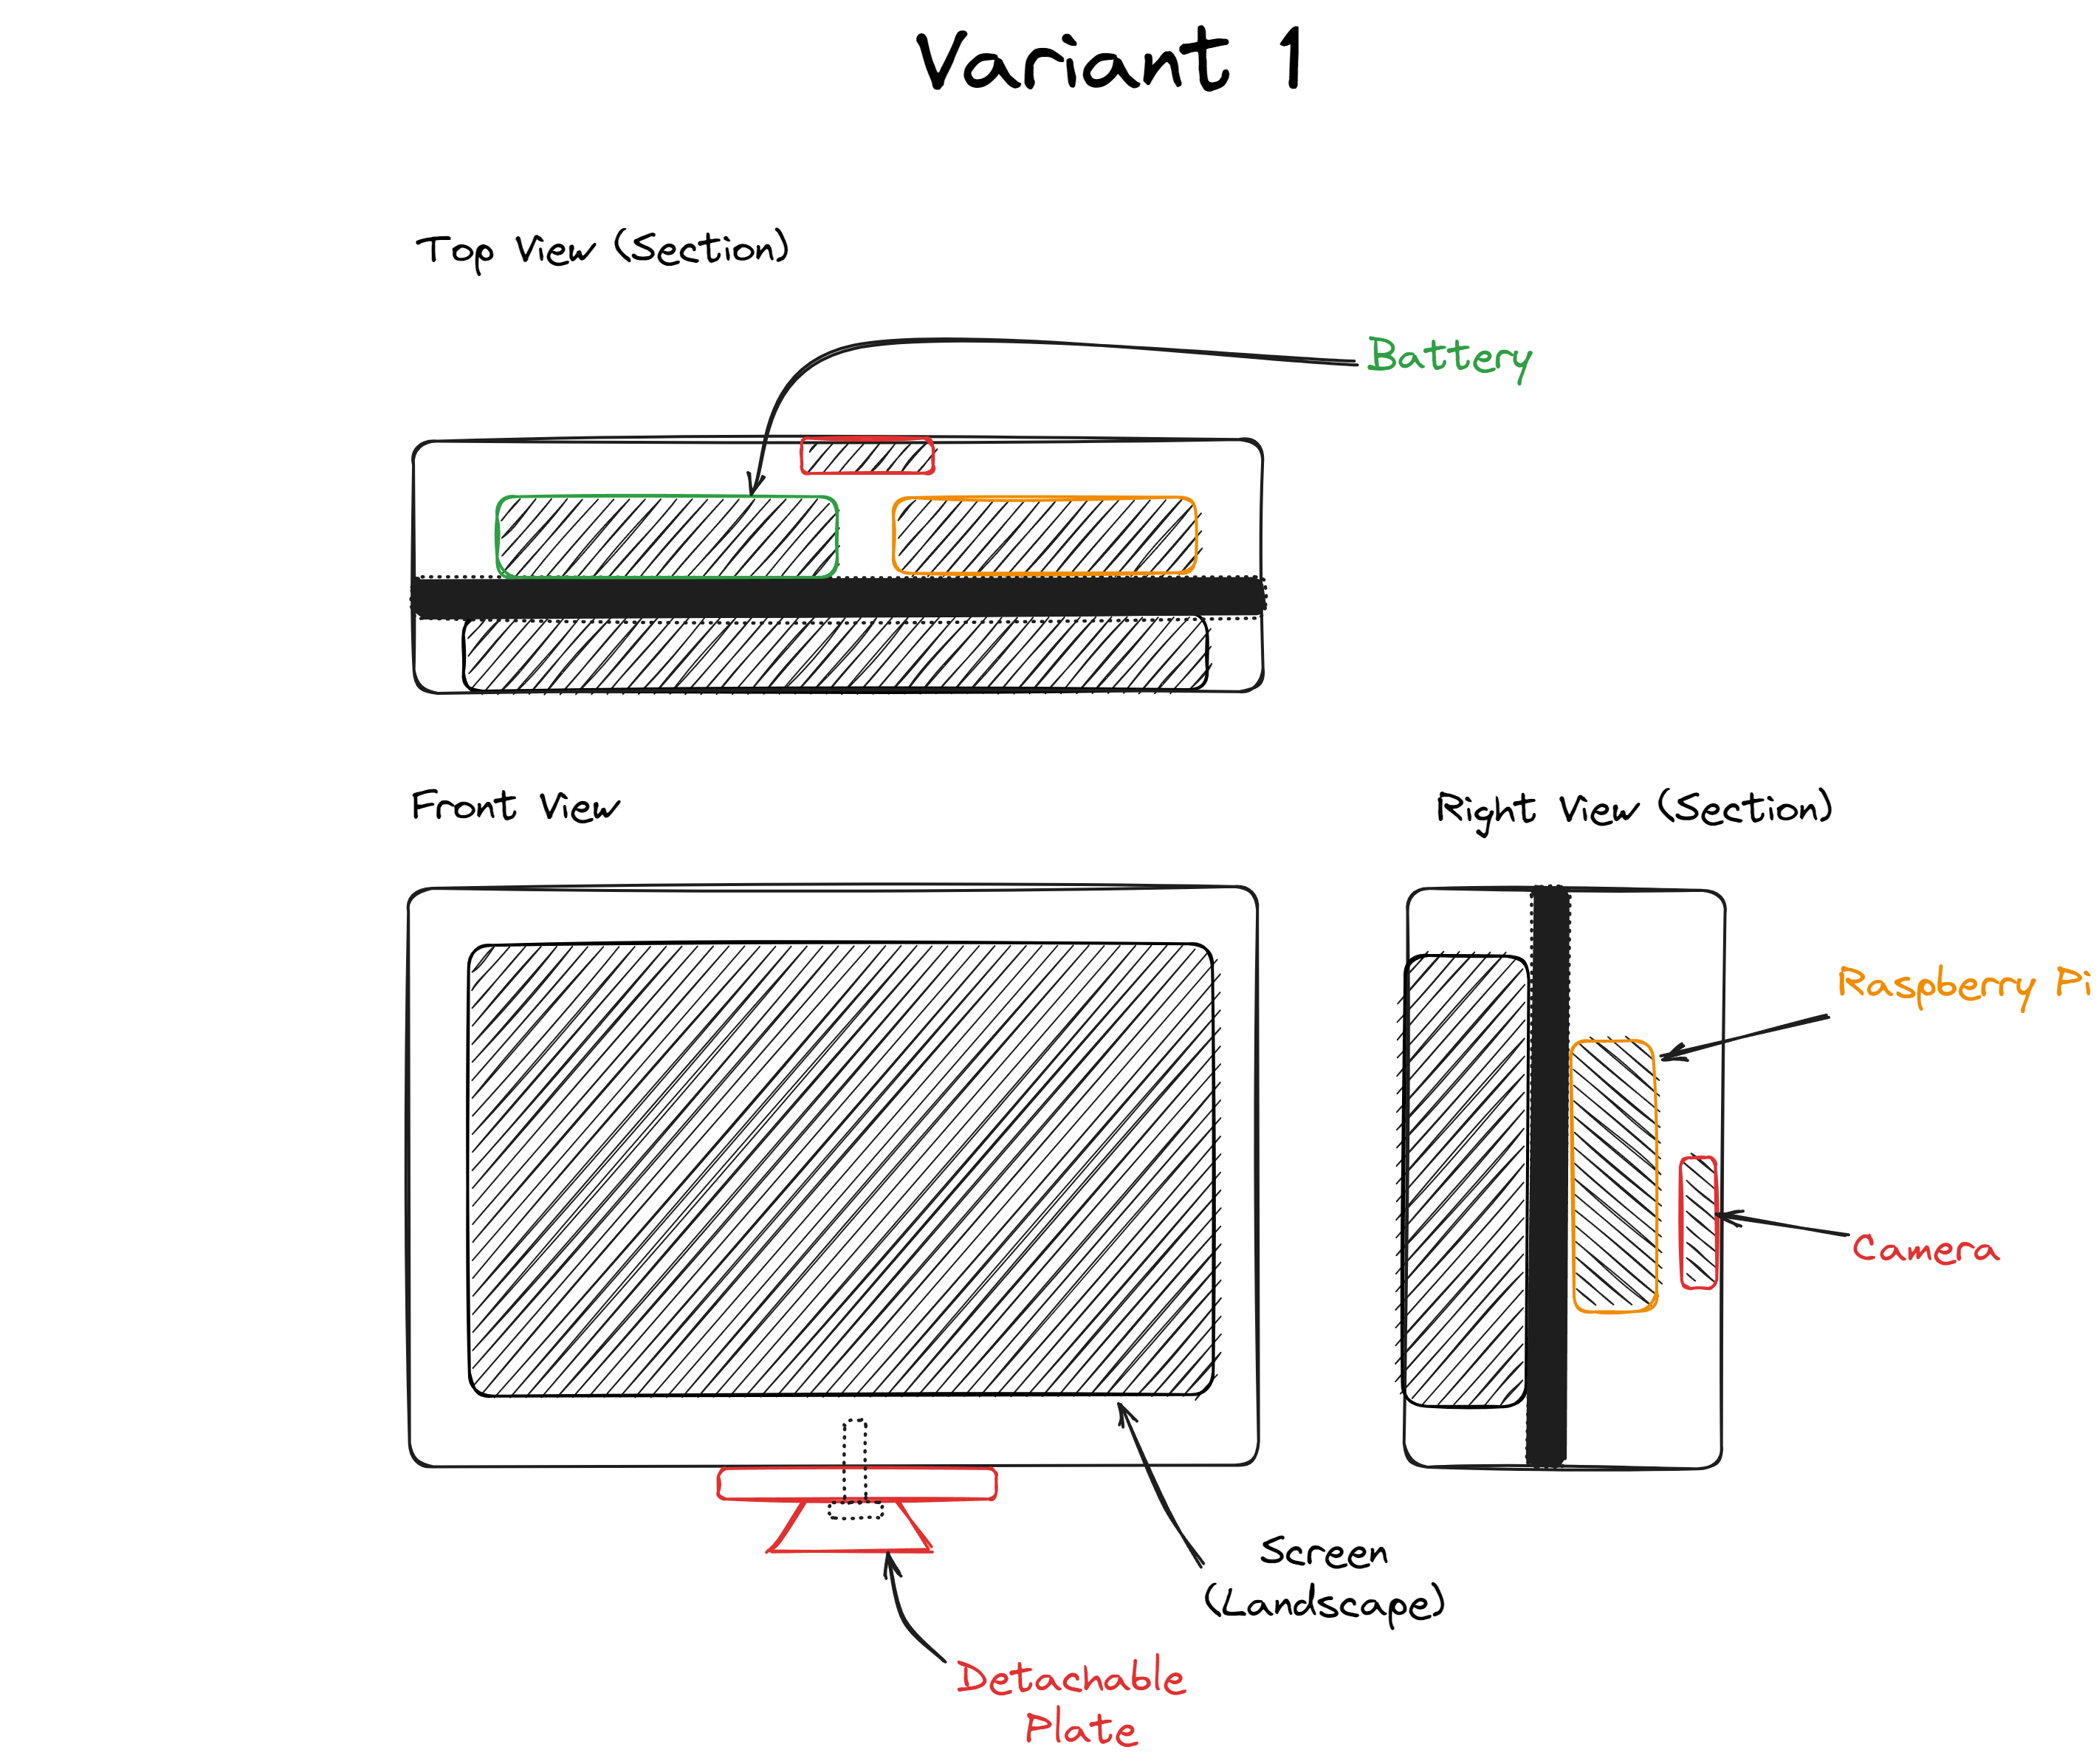
\includegraphics[width=0.75\linewidth]{texs/Part1/chapter3/image/v1.png}
    \caption{Sketch of Solution Variant 1}
    \label{fig:sketch-solution-variant-1}
\end{figure}


\subsection{Solution Variant 2, S2}
Similar to previous variant, Solution Variant 2 maintains a tablet-like design, with components arranged like a tablet device (see Figure \ref{fig:sketch-solution-variant-2}). One significant difference lies in the control mechanism. While Solution Variant 1 relies on a touch screen, Solution Variant 2 incorporates physical buttons as the primary control mechanism. This addition enhances versatility and usability in various scenarios, as users can choose between touch-based and tactile input.

\begin{figure}[H]
    \centering
    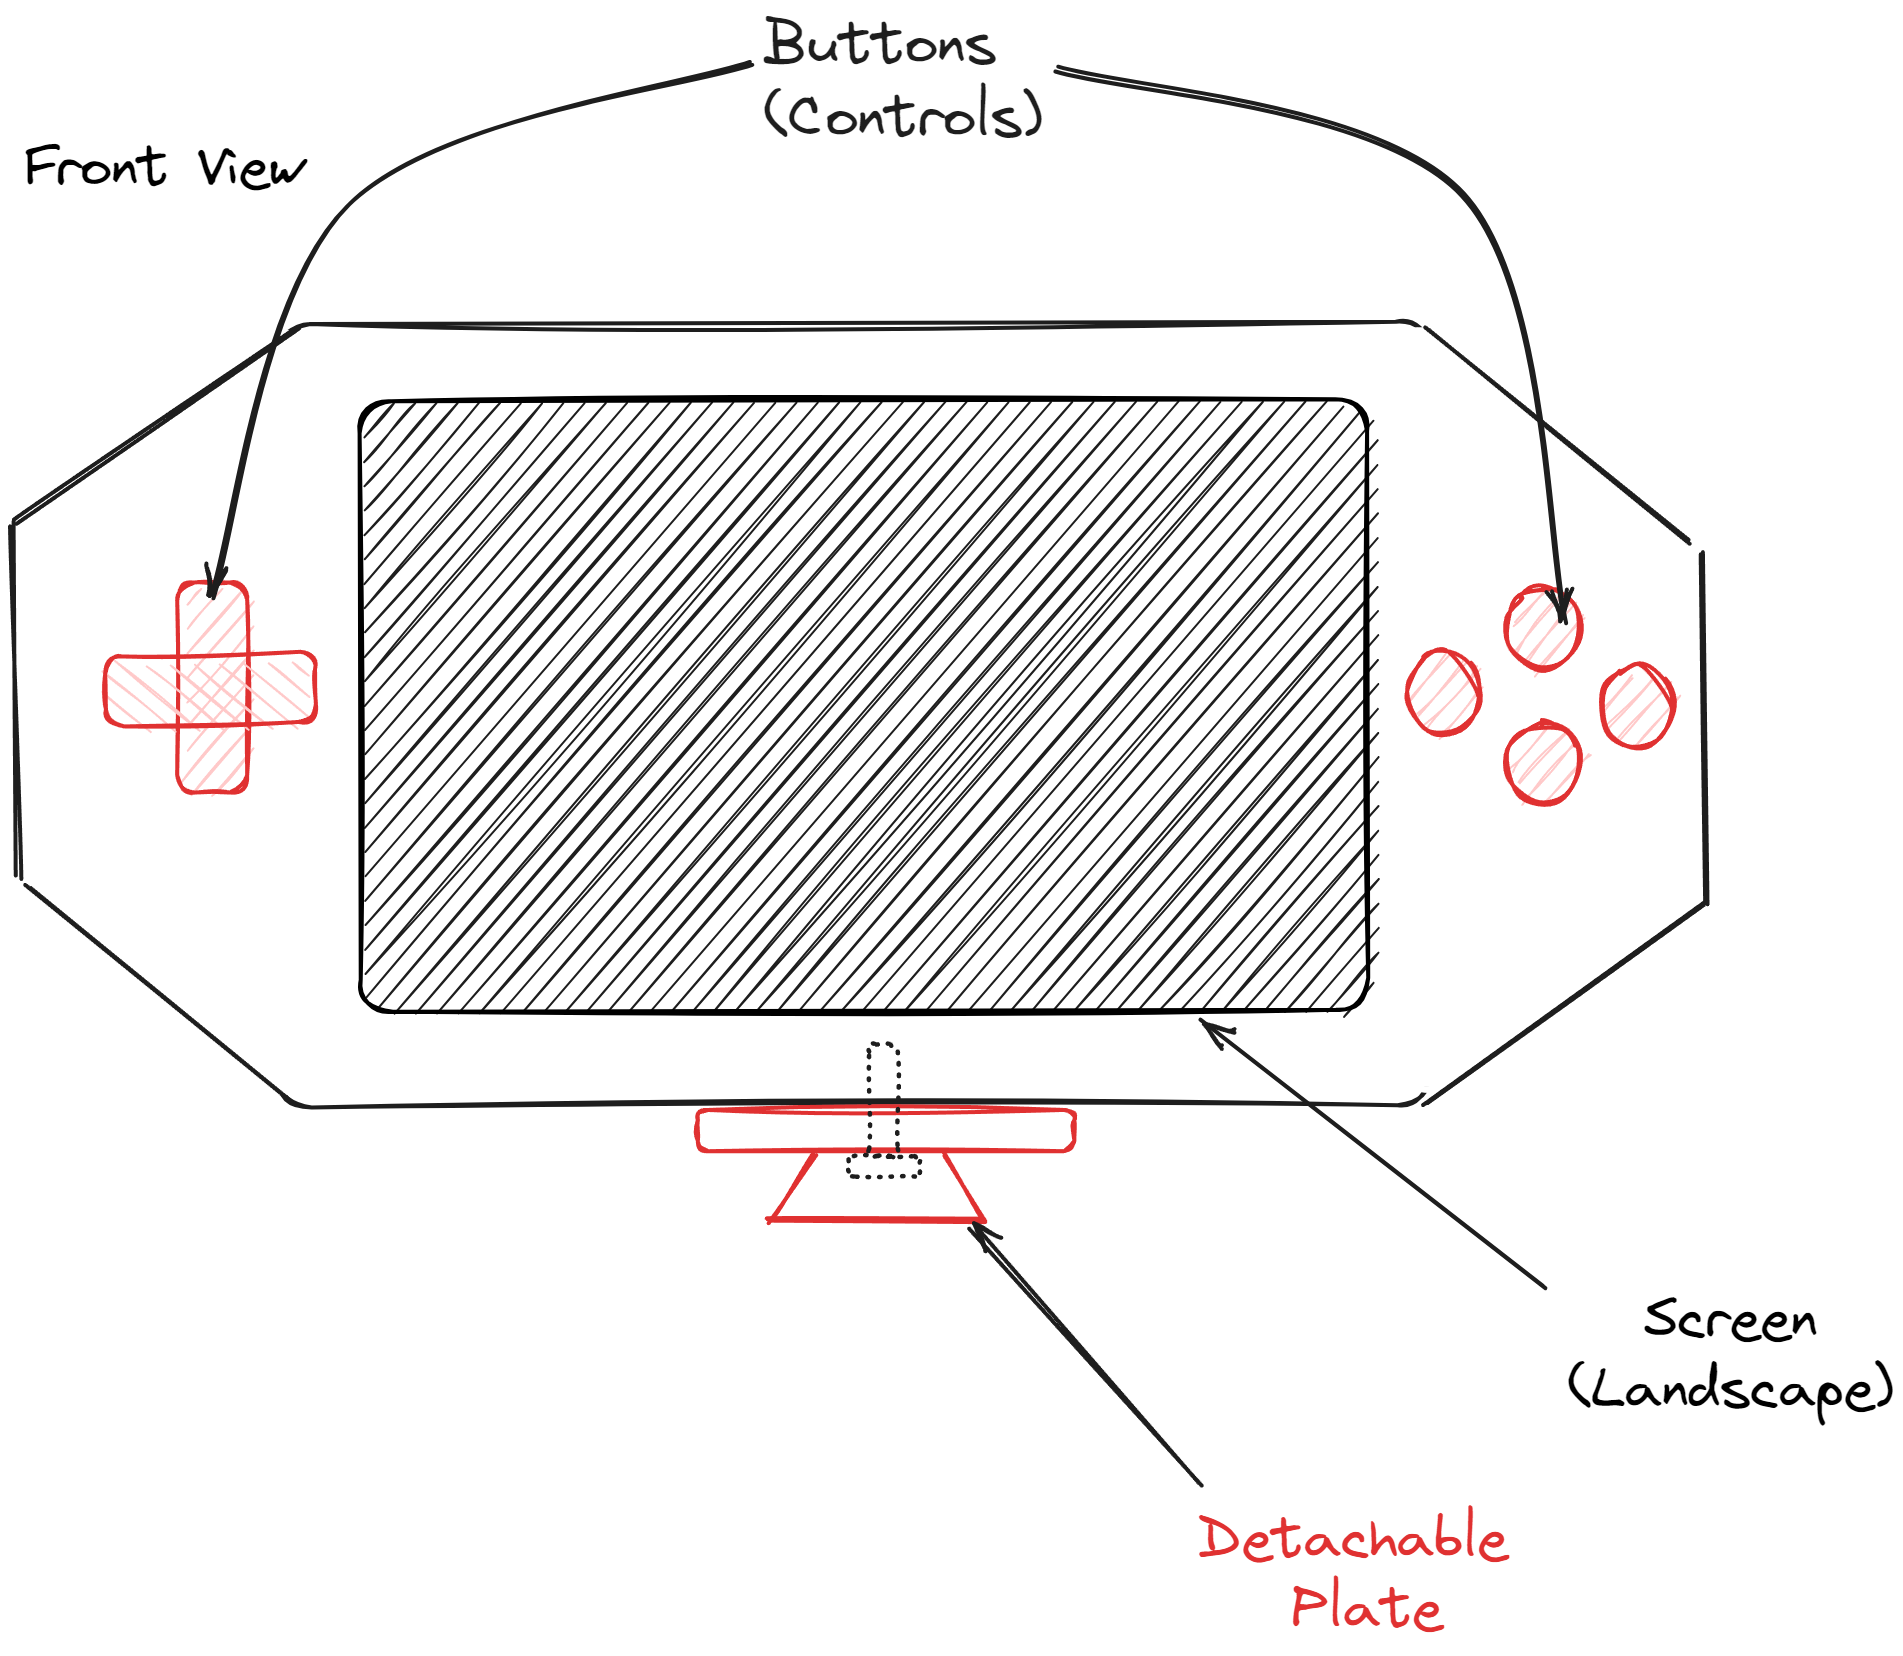
\includegraphics[width=0.55\linewidth]{texs/Part1/chapter3/image/v2.png}
    \caption{Sketch of Solution Variant 2}
    \label{fig:sketch-solution-variant-2}
\end{figure}

\subsection{Solution Variant 3, S3}
While Solution Variant 3 maintains the tablet-like component placement found in the previous variants, it introduces a significant change by adopting a portrait screen orientation. This shift opens up new possibilities for the device's usage, particularly in scenarios where vertical screen space is more advantageous than horizontal layout.

The design includes a bump grip for secure and comfortable handling in a vertical position. Notably, the battery is positioned externally in this variant, offering the potential advantage of easier access and replacement. The body structure remains a sandwich-type, providing robust protection for the internal components.

One notable advantage of the portrait screen orientation is the improved stability of the device, as the center of gravity is aligned with the device's center. This alignment enhances balance and control when using the device in various orientations, thus enhancing overall usability and versatility.

\begin{figure}[H]
    \centering
    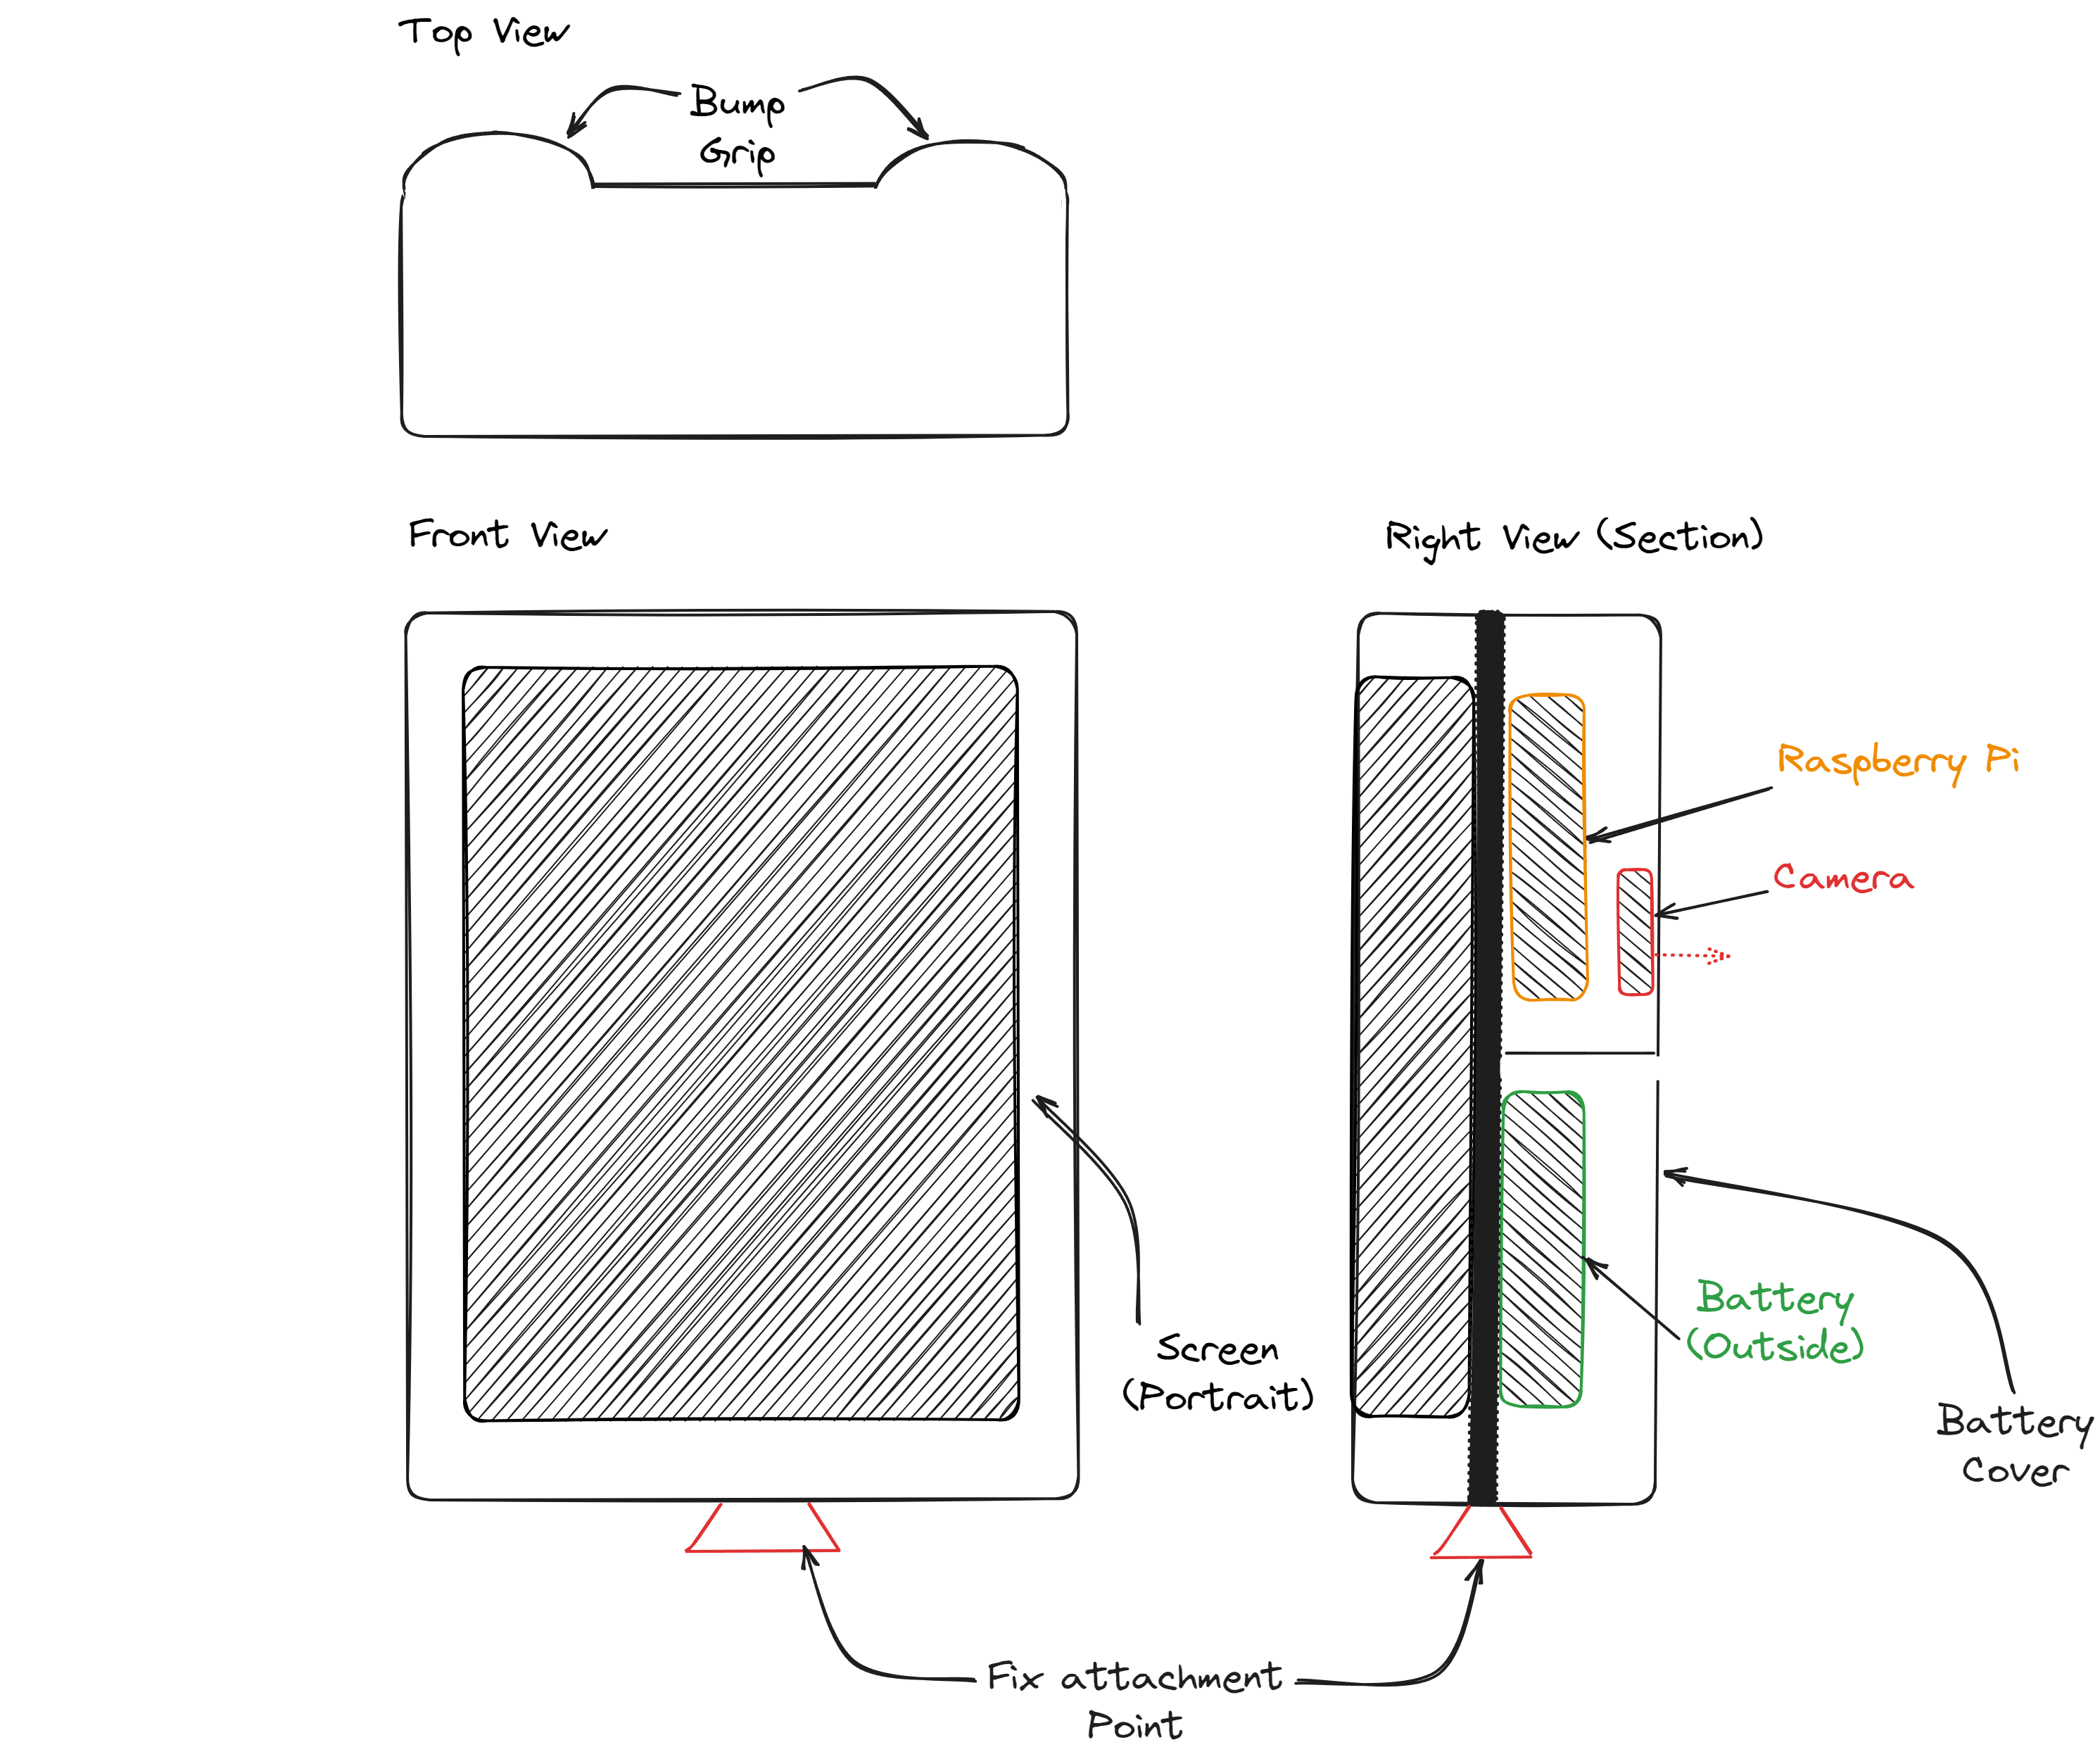
\includegraphics[width=0.75\linewidth]{texs/Part1/chapter3/image/v3.png}
    \caption{Sketch of Solution Variant 3}
    \label{fig:sketch-solution-variant-3}
\end{figure}

\subsection{Solution Variant 4, S4}
Solution Variant 4 copies many features from Solution Variant 3, but with one significant change in the body type. Solution Variant 4 opts for a more minimalistic skeleton design, which results in a lightweight yet adequately supportive body for the internal components. This design choice is particularly beneficial for users who prefer a lightweight device for extended usage periods. Figure \ref{fig:sketch-solution-variant-4} shows the sketch of Solution Variant 4.

\begin{figure}[H]
    \centering
    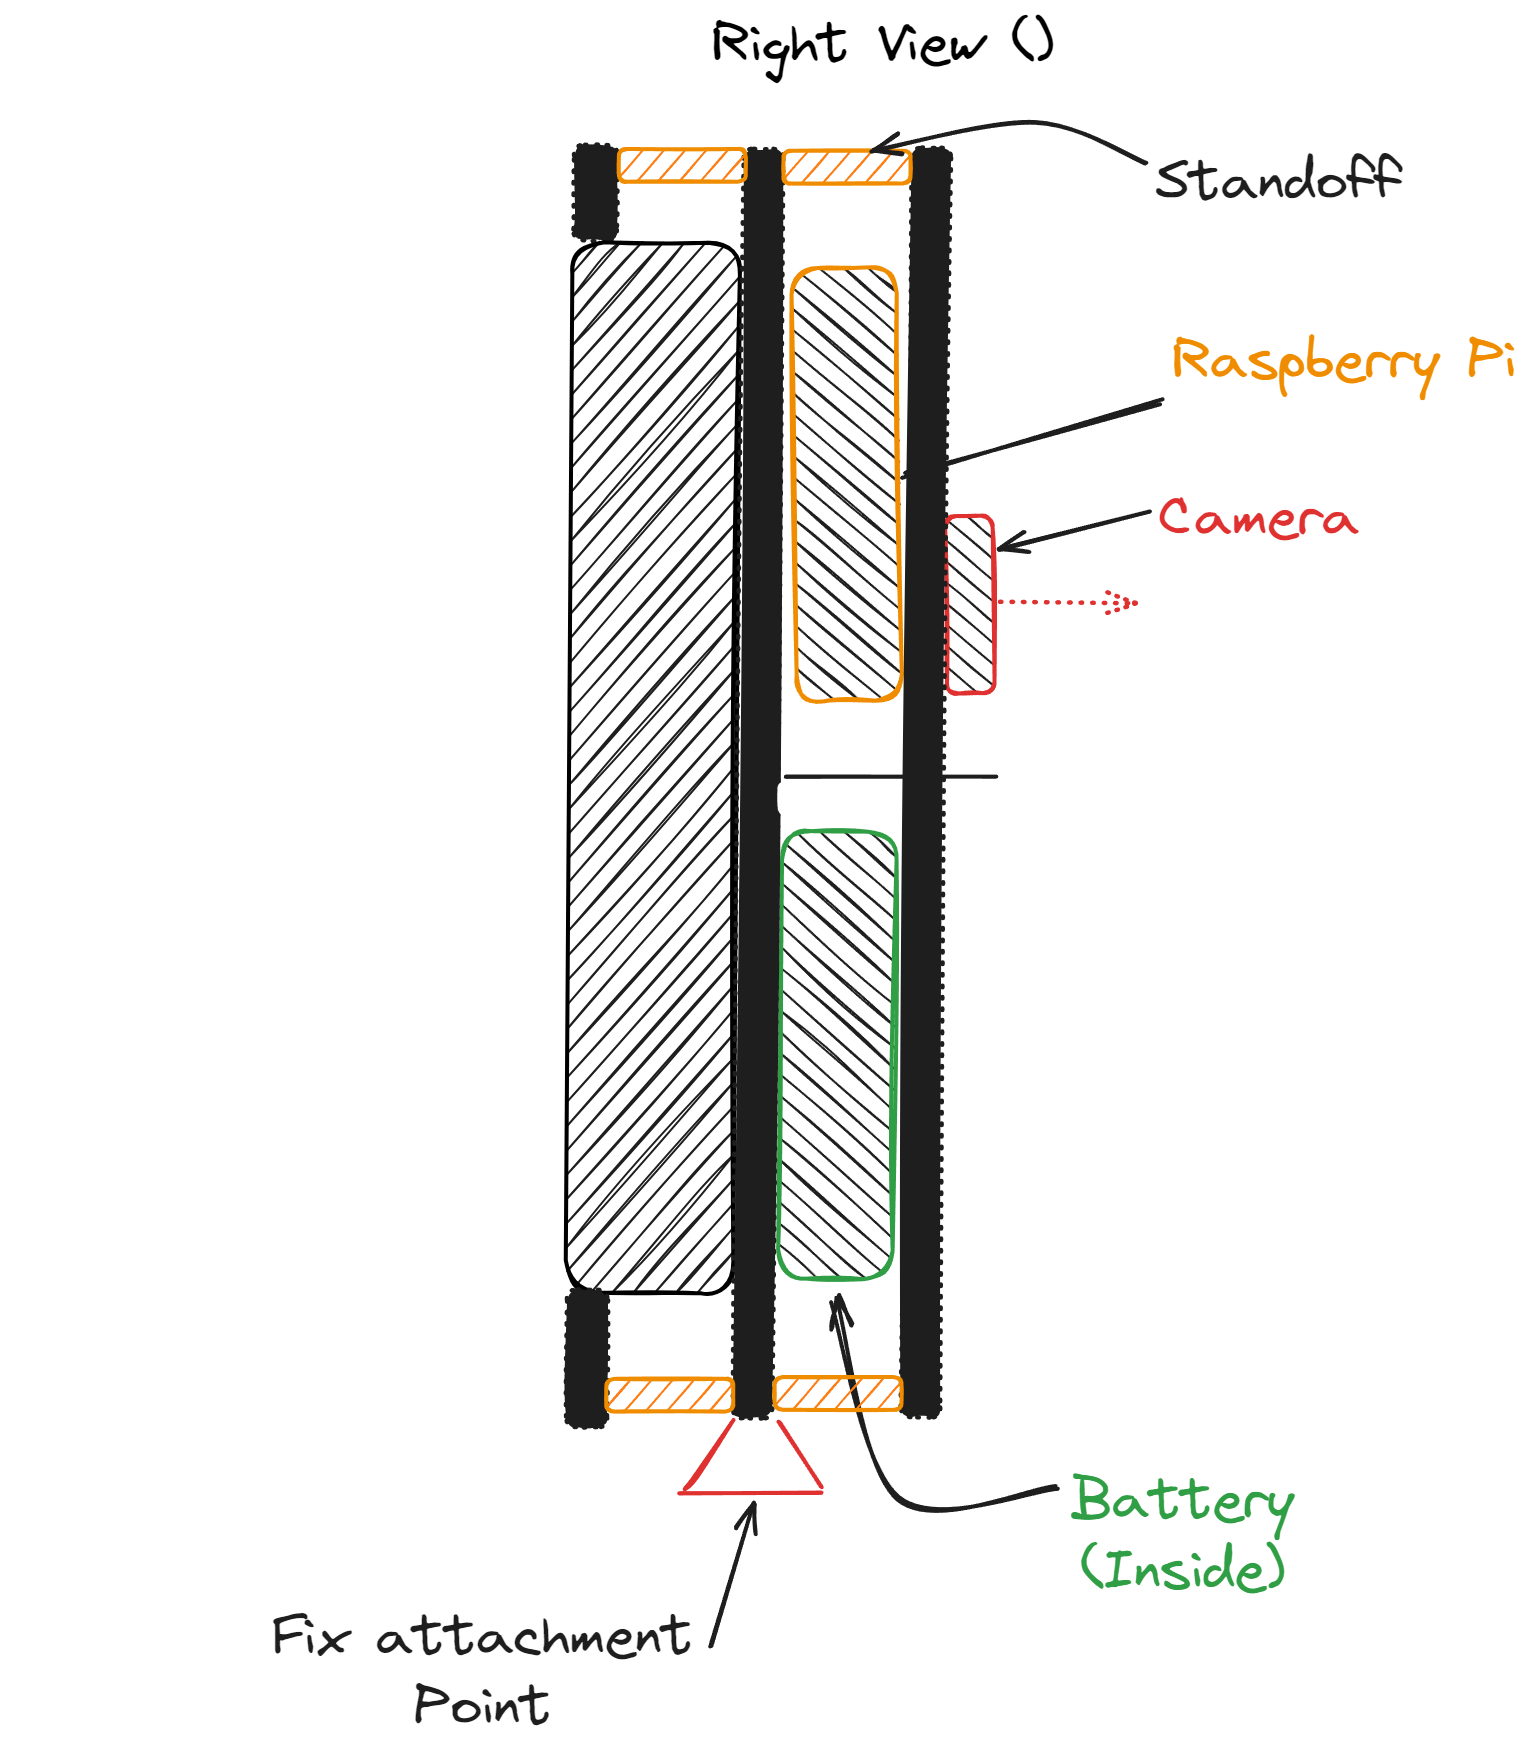
\includegraphics[width=0.5\linewidth]{texs/Part1/chapter3/image/v4.png}
    \caption{Sketch of Solution Variant 4}
    \label{fig:sketch-solution-variant-4}
\end{figure}

\subsection{Solution Variant 5, S5}
Solution Variant 5 introduces a unique design approach, deviating from the tablet-like structure seen in previous solutions. Instead, it adopts a Point of Service-like component placement, where the Raspberry Pi, Battery, Camera, and Screen are configured in a distinctive layout. The screen is positioned at an angle, differentiating it from the previous variants (see Figure \ref{fig:sketch-solution-variant-5}).

Regarding screen orientation, Solution Variant 5 retains a portrait mode, which can be advantageous in scenarios requiring vertical displays. The device is designed for body grip handling, offering a secure way to hold and interact with the device.

A notable difference is the external AAA battery setup, which enhances convenience by offering easy battery replacement and compatibility with standard batteries. The body structure follows the familiar sandwich-type design, providing robust protection for the internal components.

For mounting purposes, Solution Variant 5 utilizes the detachable tripod system, enabling seamless attachment and detachment from a tripod stand. Like its predecessors, it relies on a touch screen as the primary control mechanism, ensuring intuitive user interactions.

\begin{figure}[H]
    \centering
    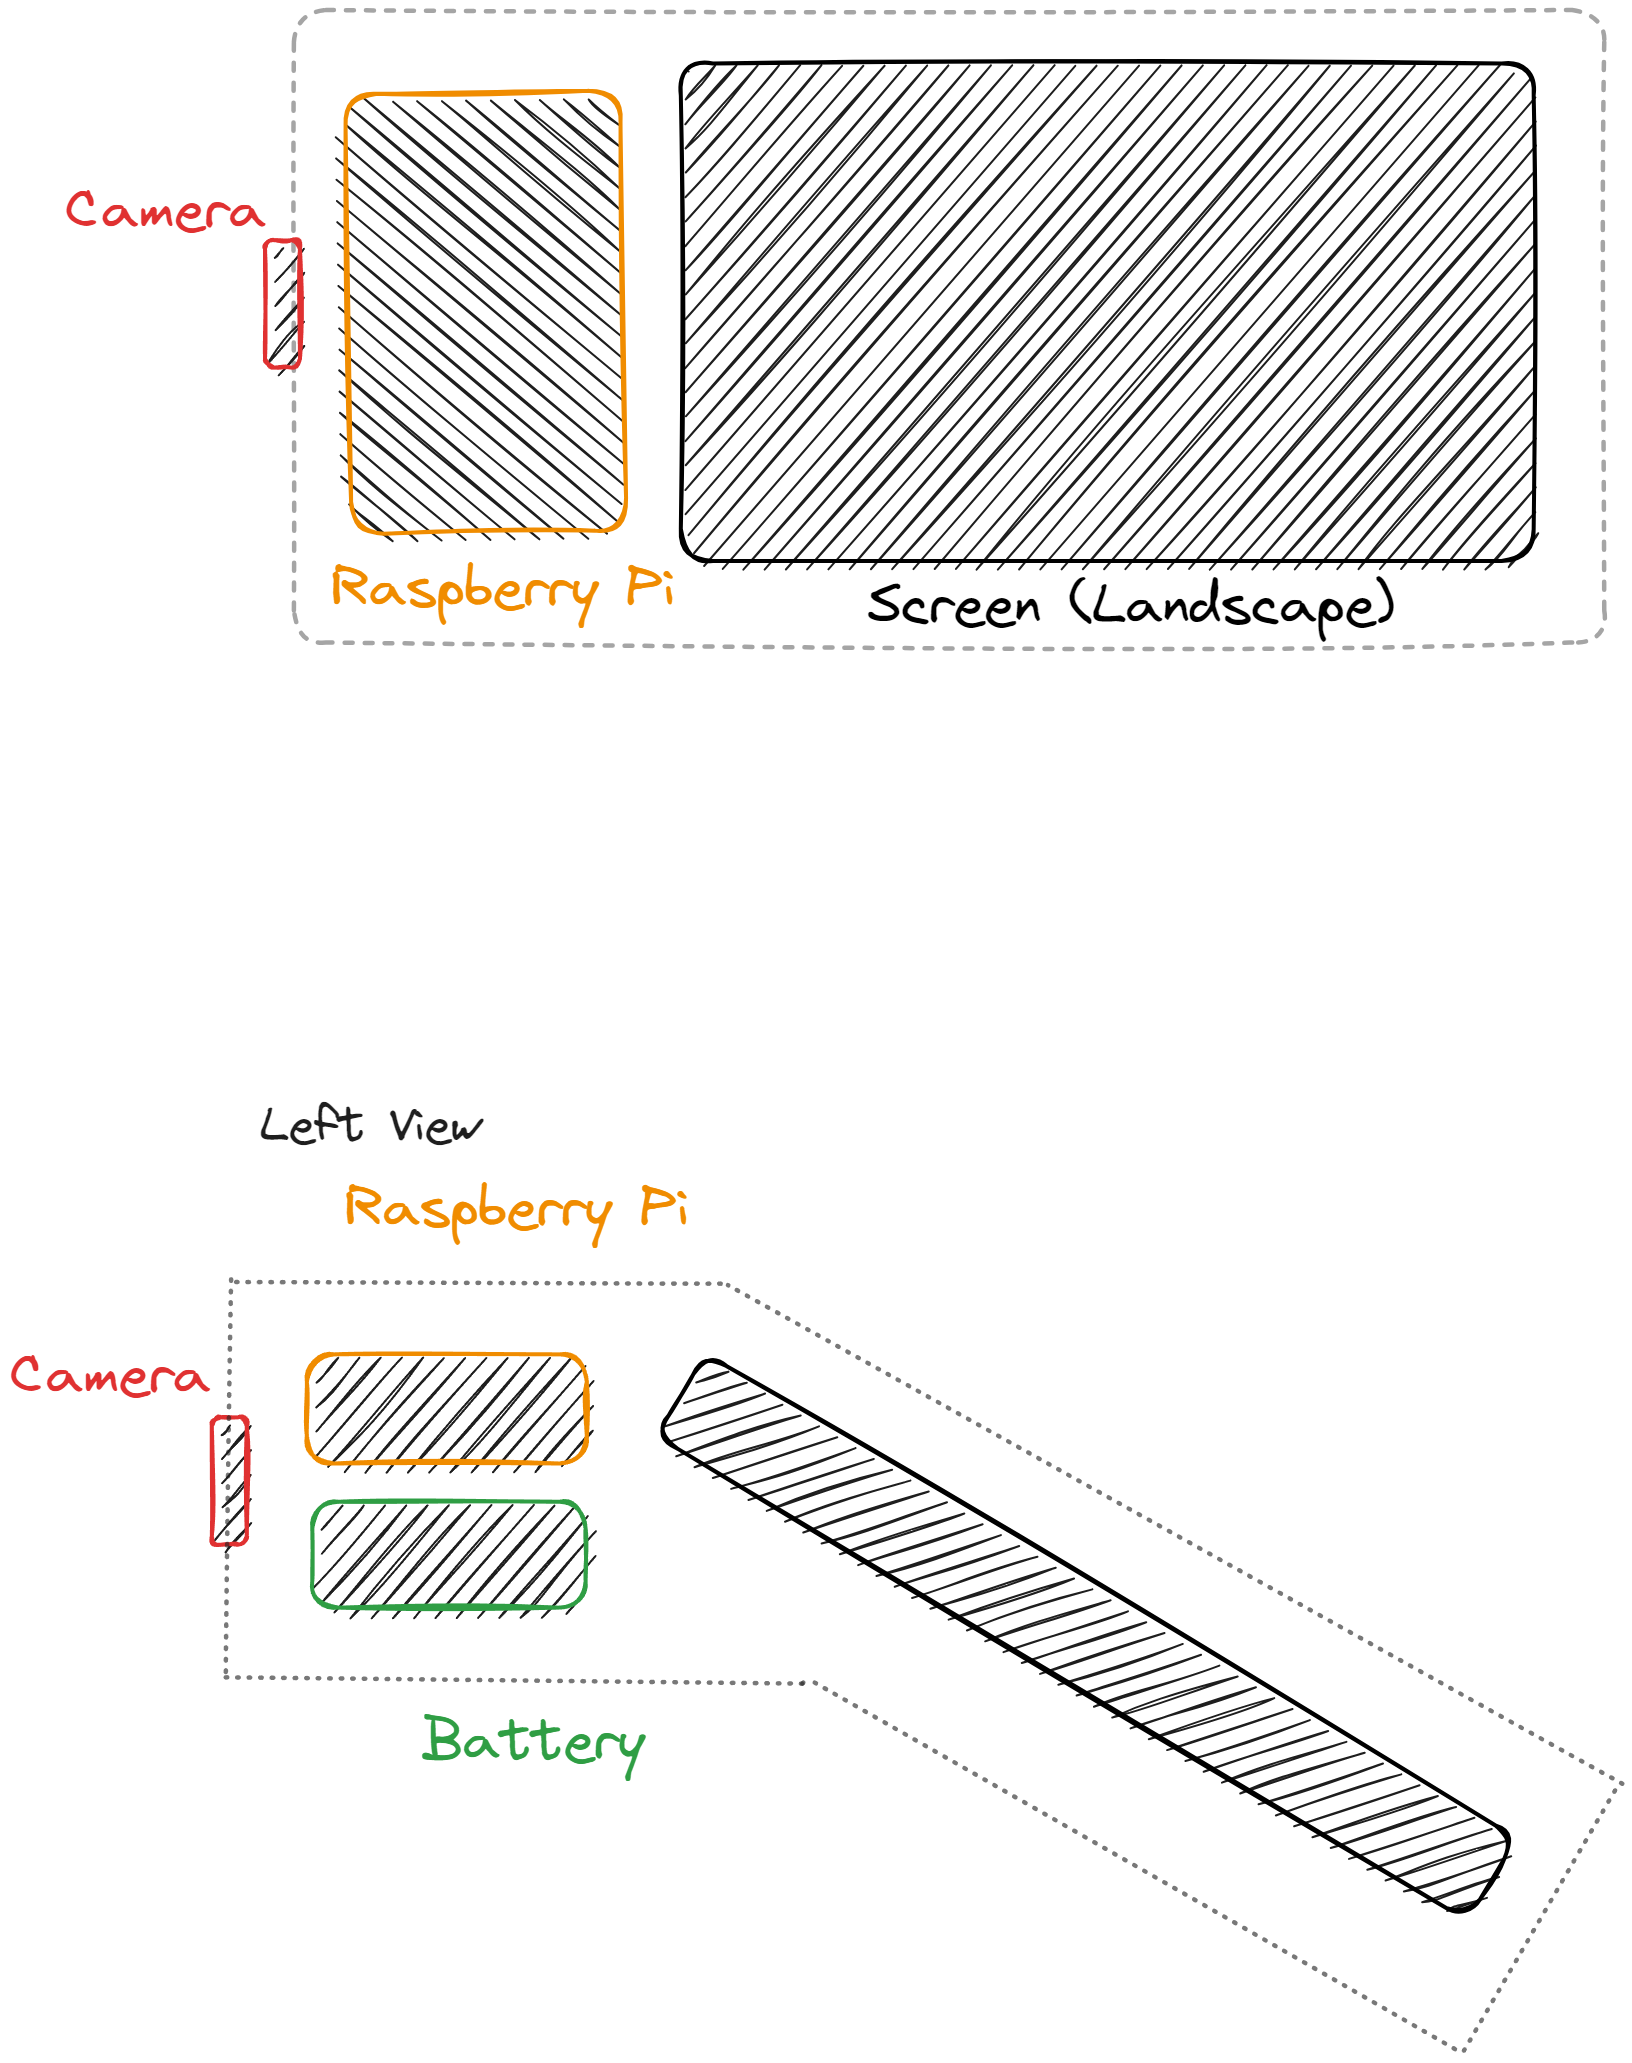
\includegraphics[width=0.5\linewidth]{texs/Part1/chapter3/image/v5.png}
    \caption{Sketch of Solution Variant 5}
    \label{fig:sketch-solution-variant-5}
\end{figure}

\subsection{Solution Variant 6, S6}
Solution Variant 6 closely mirrors Solution Variant 5 regarding component placement and screen orientation. This variant, too, adopts the Point of Service-like layout with a portrait screen orientation. However, it introduces a pistol handle for handling, providing a firm and ergonomic grip for users, as can be seen in Figure \ref{fig:sketch-solution-variant-6}.

The battery is positioned externally, offering the same benefits of easy battery replacement and extended usage periods. Regarding body design, Solution Variant 6 employs a bowl-like structure with all components attached to the main body. This design choice provides protection and enclosure while reducing overall weight.

\begin{figure}[H]
    \centering
    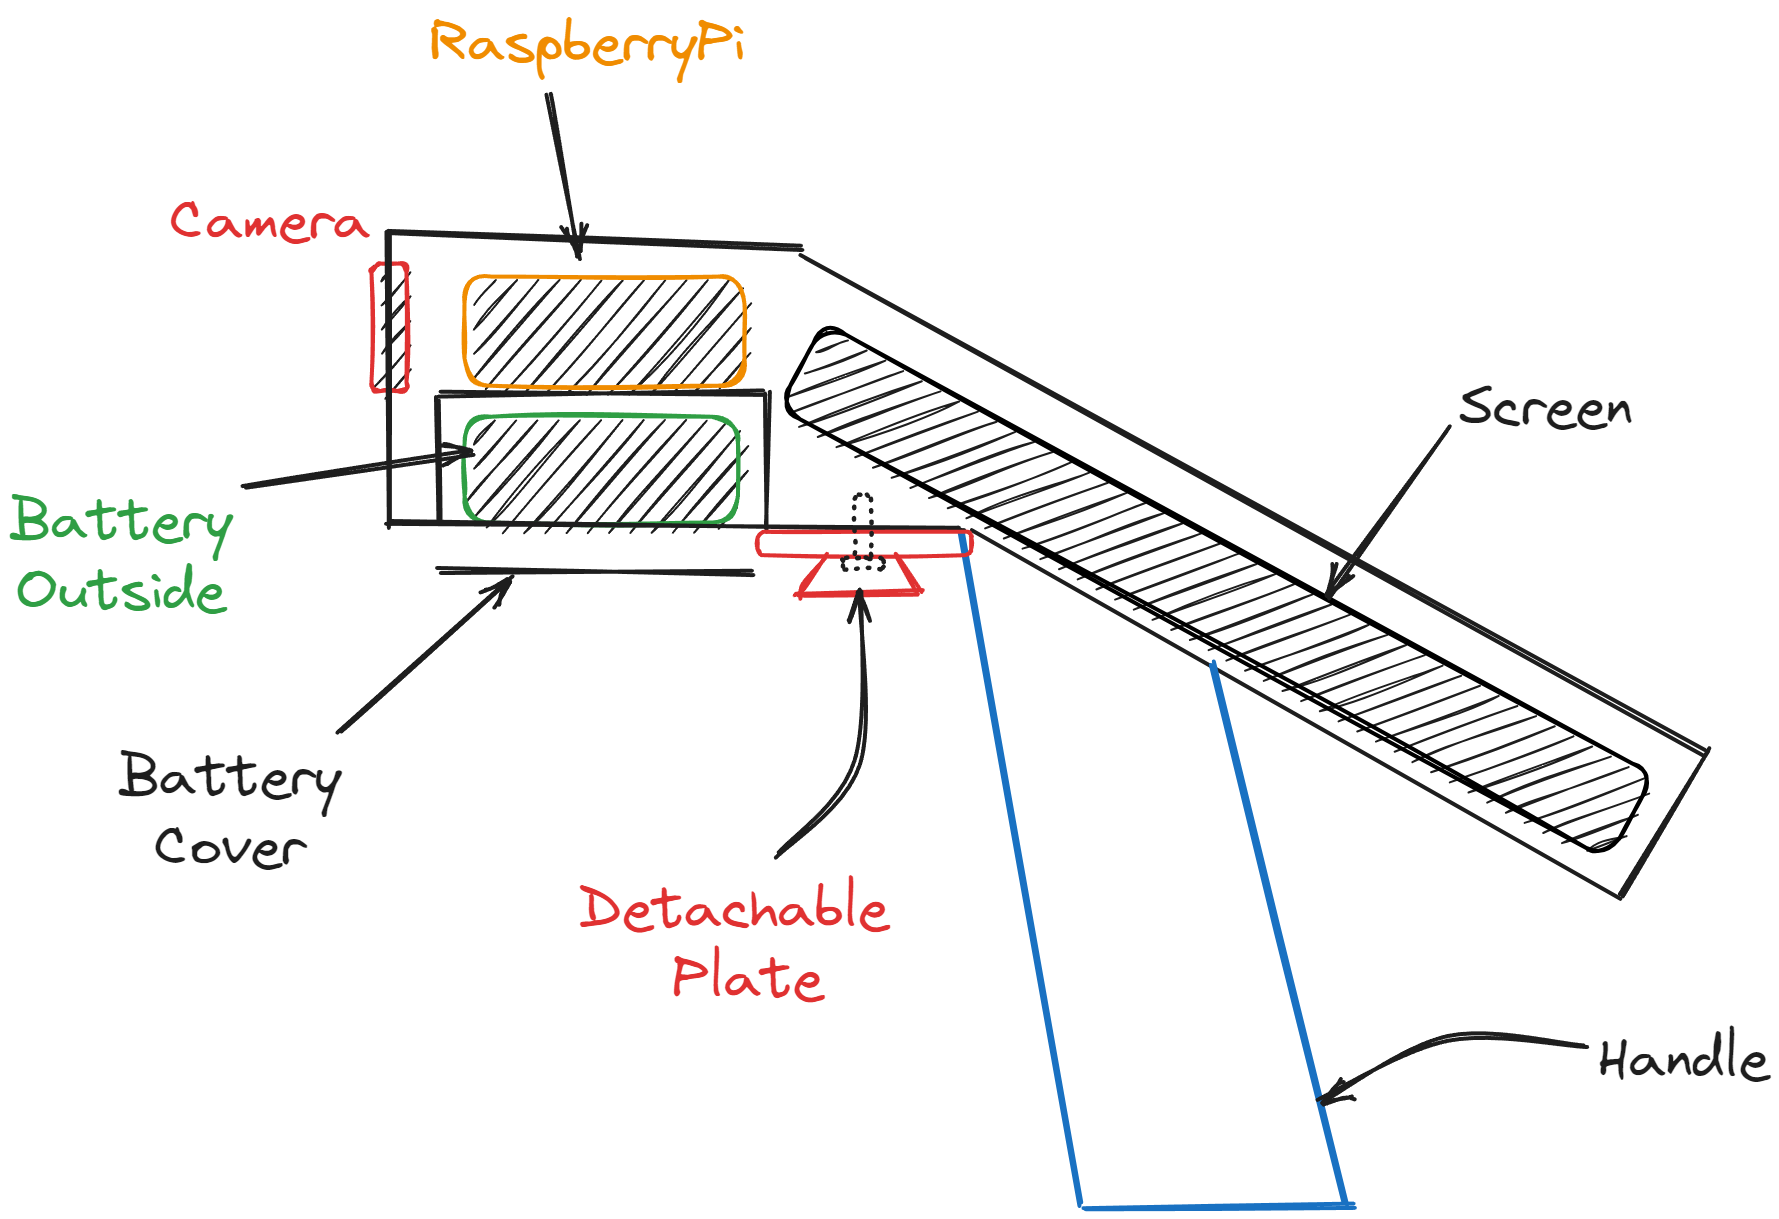
\includegraphics[width=0.5\linewidth]{texs/Part1/chapter3/image/v6.png}
    \caption{Sketch of Solution Variant 6}
    \label{fig:sketch-solution-variant-6}
\end{figure}

\subsection{Solution Variant 7, S7}
In Solution Variant 7, a distinct design approach with a Handheld PC-like component placement is produced. This configuration aligns the screen and battery, positioning the Raspberry Pi behind the screen (see Figure \ref{fig:sketch-solution-variant-7}).

The variant is specifically designed with a bump grip, providing a secure and comfortable handling experience. Additionally, a rounded battery can be used within this variant and placed inside the bump grip. This design has the potential to offer a more streamlined and integrated appearance.

The chassis structure adopts a bowl-like design, ensuring secure enclosure and protection for all components. The device incorporates a built-in tripod system for mounting, providing a stable attachment to a tripod stand.

Solution Variant 7 combines a touch screen and physical buttons as the control mechanism. This dual-input approach provides users multiple options for interacting with the device's functionalities, enhancing versatility and usability in various scenarios.

\begin{figure}[H]
    \centering
    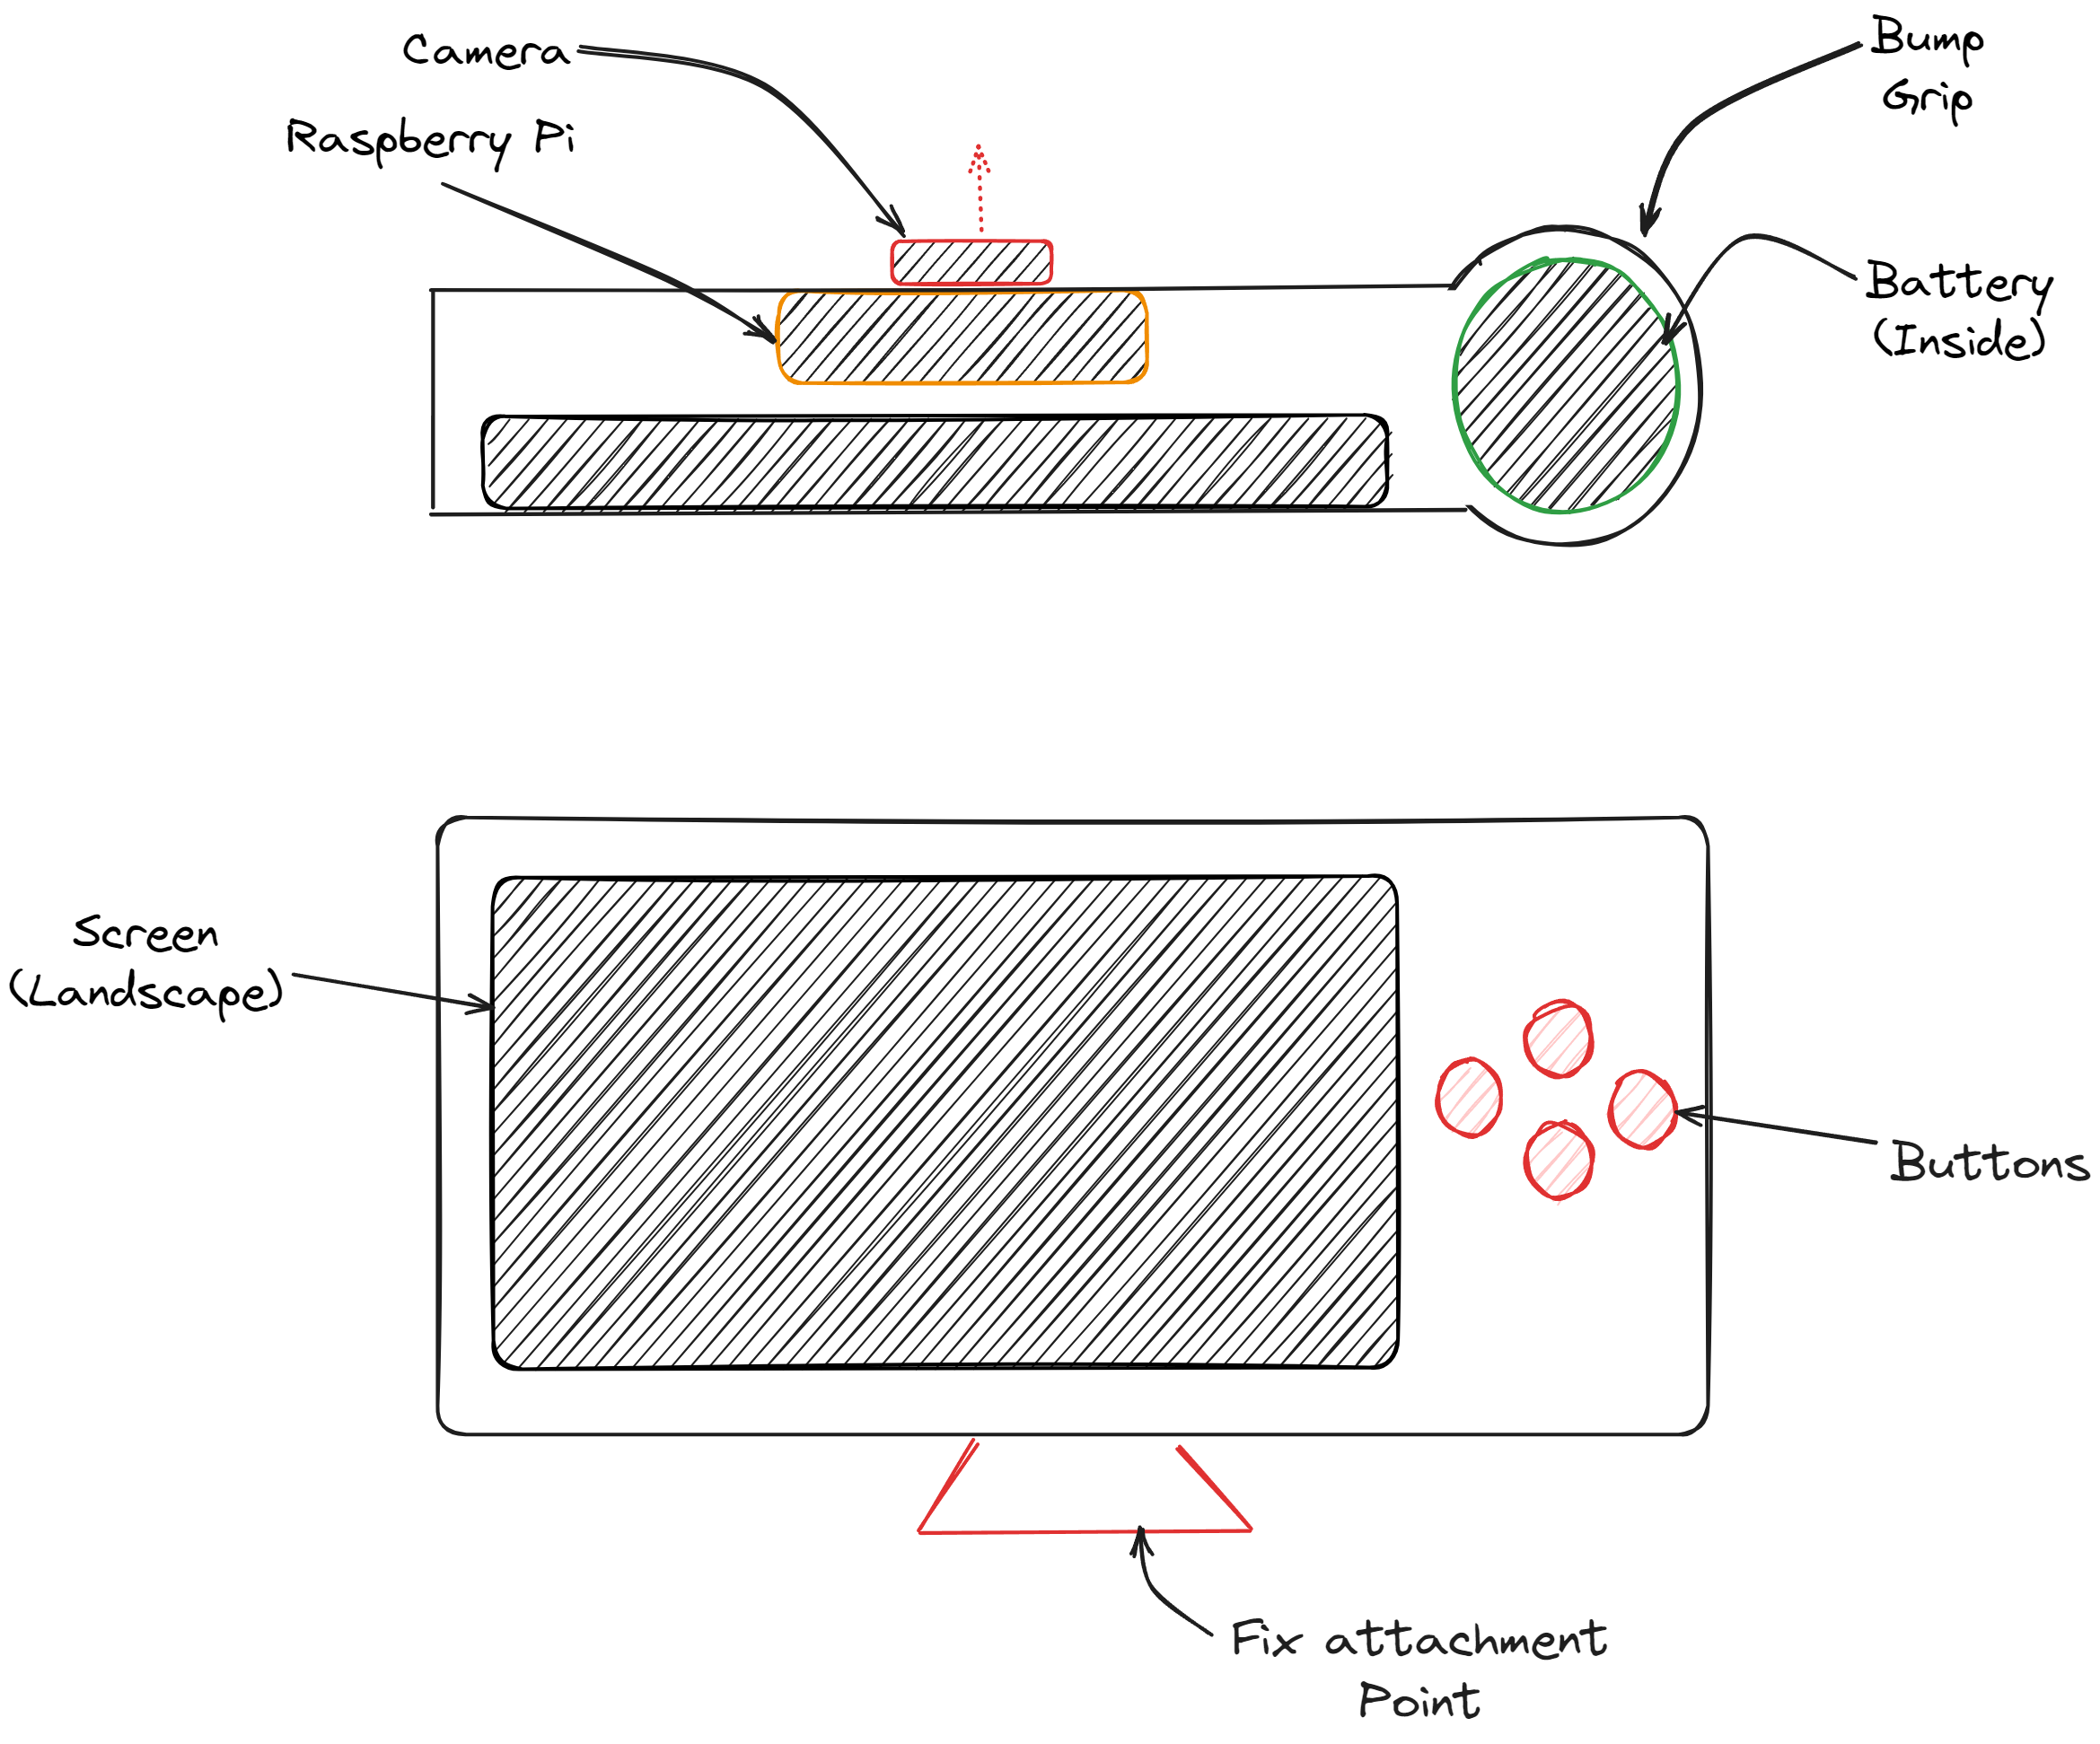
\includegraphics[width=0.5\linewidth]{texs/Part1/chapter3/image/v7.png}
    \caption{Sketch of Solution Variant 7}
    \label{fig:sketch-solution-variant-7}
\end{figure}

\subsection{Solution Variant 8, S8}
Solution Variant 8 features a Camcorder-like component placement. The Raspberry Pi, Battery, Camera, and Screen are arranged similarly to a camcorder, with the screen positioned at a hinge, allowing it to change angles for flexible viewing.

The screen orientation remains landscape, providing a broad horizontal display view. The device is designed with a body grip for secure and comfortable handling. The battery is placed internally, and a power bank is used to provide a reliable power source.

The chassis structure follows a bowl-like design, offering protection and sturdiness for the internal components. A fixed-mount tripod system is employed for mounting purposes, providing stability and ease of use when attaching the device to a tripod stand.

As with some of the previous variants, Solution Variant 8 combines both a touch screen and physical buttons as the control mechanism, offering users the flexibility to interact.

\begin{figure}[H]
    \centering
    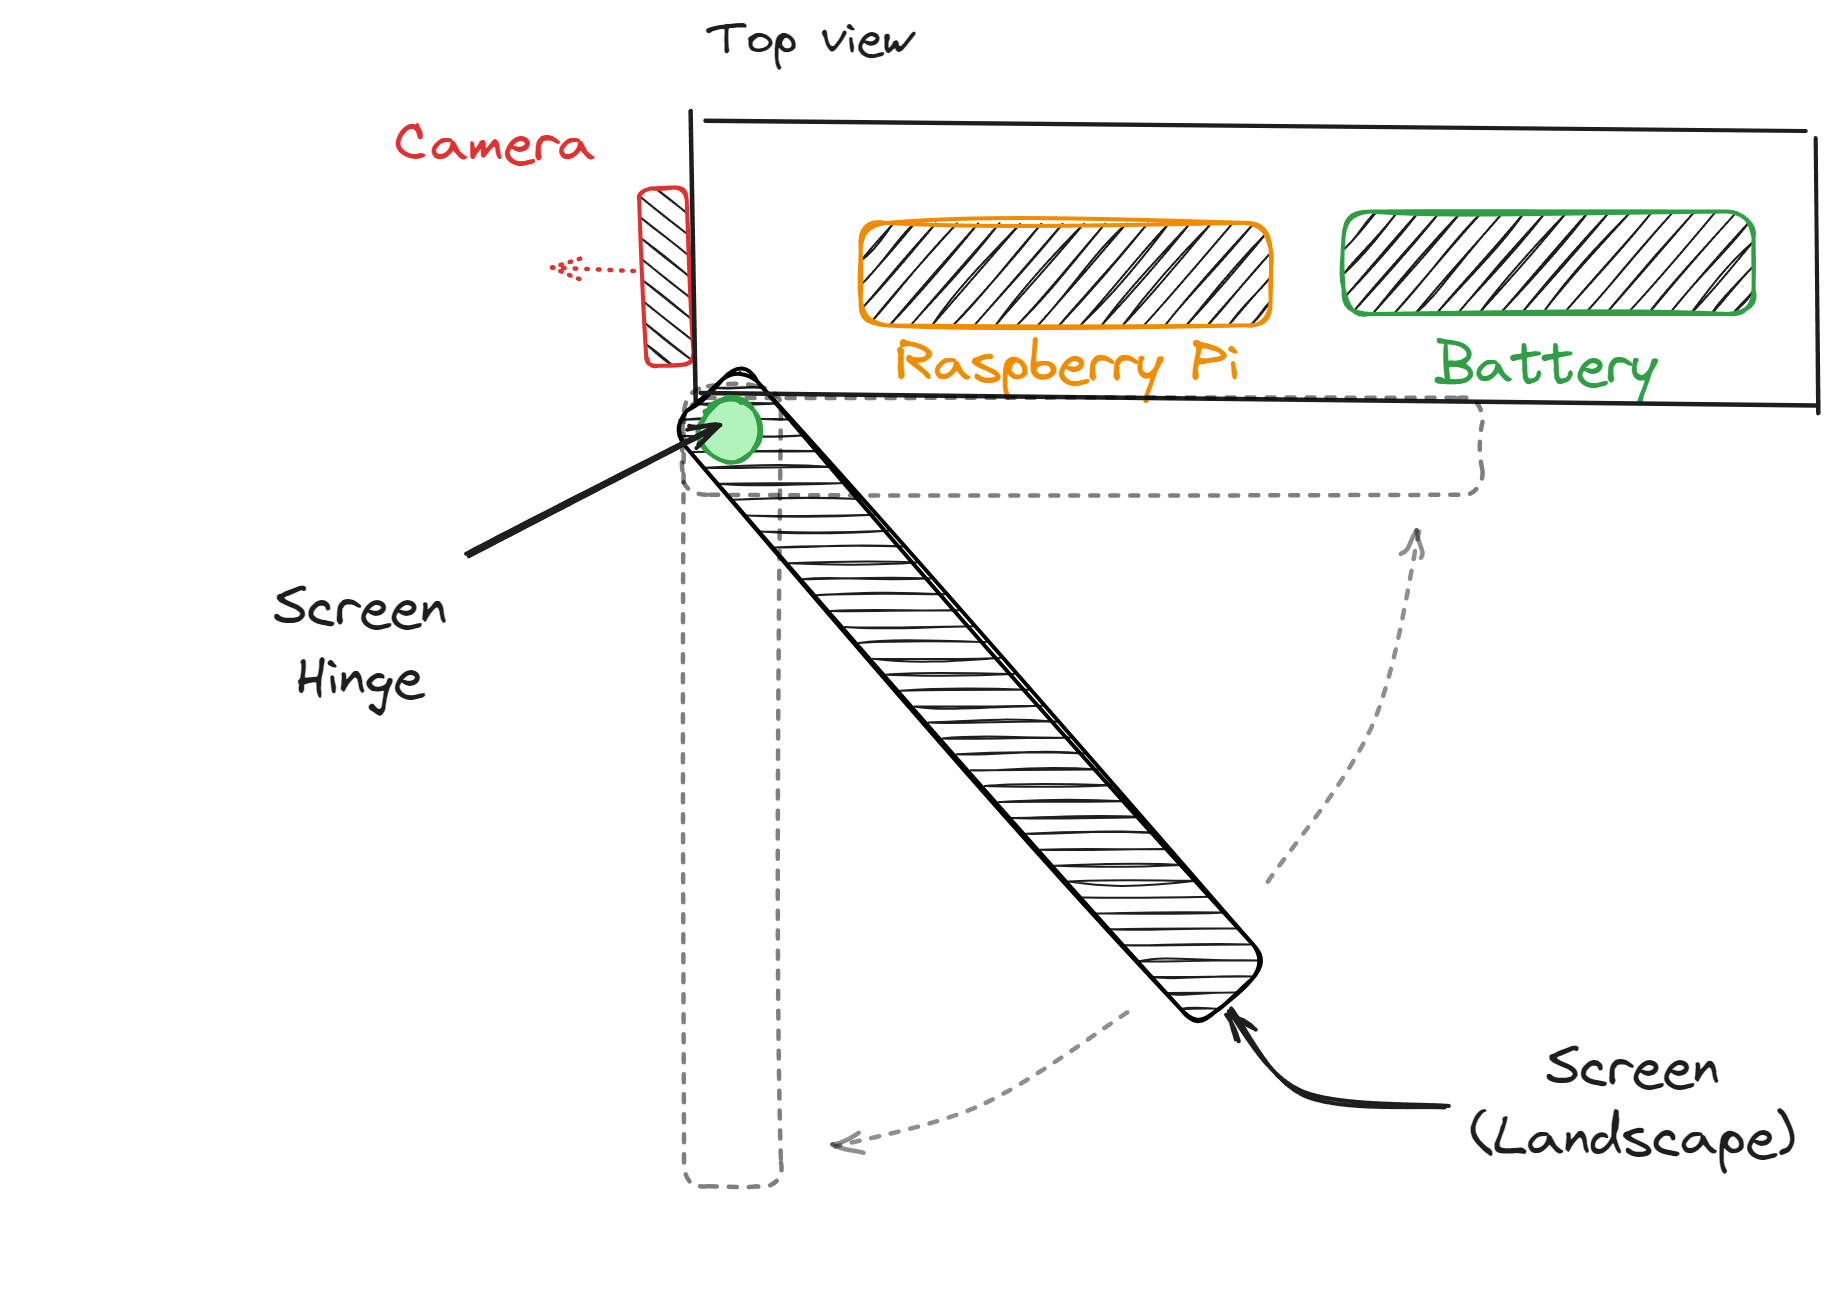
\includegraphics[width=0.5\linewidth]{texs/Part1/chapter3/image/v8.png}
    \caption{Sketch of Solution Variant 8}
    \label{fig:sketch-solution-variant-8}
\end{figure}

\section{Filtering of Solution Variants}
\label{sec:filtering-of-solution-variants}
As shown in Figure \ref{fig:morphological-chart-with-solution-variants}, multiple solution variants were generated. However, not all of these solutions are feasible and practical. As advised by Pahl and Beitz \cite[106-107]{Pahl2007}, it is necessary to reduce the vast number of theoretically possible but practically unachievable solutions as early as possible. However, caution should be exercised not to discard valuable working principles, as they often play a crucial role in forming a favorable and effective working structure when combined with others.

Additionally, Pahl and Beitz \cite[107]{Pahl2007} suggest a method that can be used to filter the solution variants. This method is known as the selection chart, which consists of two steps: elimination and preference. Initially, all clearly unsuitable proposals are removed. If a substantial number of solutions remain, preference is given to those who stand out as markedly superior. Only these preferred solutions are evaluated during the final stages of the conceptual design phase.

Pahl and Beitz suggest the following criteria for eliminating unsuitable solutions:
\begin{itemize}
    \item \textbf{Criteria A:} Compatible with the overall task
    \item \textbf{Criteria B:} Fulfill demands of requirement list
    \item \textbf{Criteria C:} Realisable in principle
    \item \textbf{Criteria D:} Within permissible cost
\end{itemize}

These criteria are applied step by step to examine each solution. If any of the exclusion criteria are not met, the solution is rejected, and further criteria are not assessed. Additionally to the exclusion criteria, the following preference criteria are used to prioritize the remaining solutions:

\begin{itemize}
    \item \textbf{Criteria E:} Incorporates direct safety measures
    \item \textbf{Criteria F:} Preferred by the designer
\end{itemize}

Criteria E and F are then used to prioritize solutions if there are still too many options after the initial screening. The remarks column provides explanations for excluding or favoring each solution. The final assessment of the functional principles is recorded in the rightmost column of the selection list.

\begin{figure}[ht!]
    \centering
    {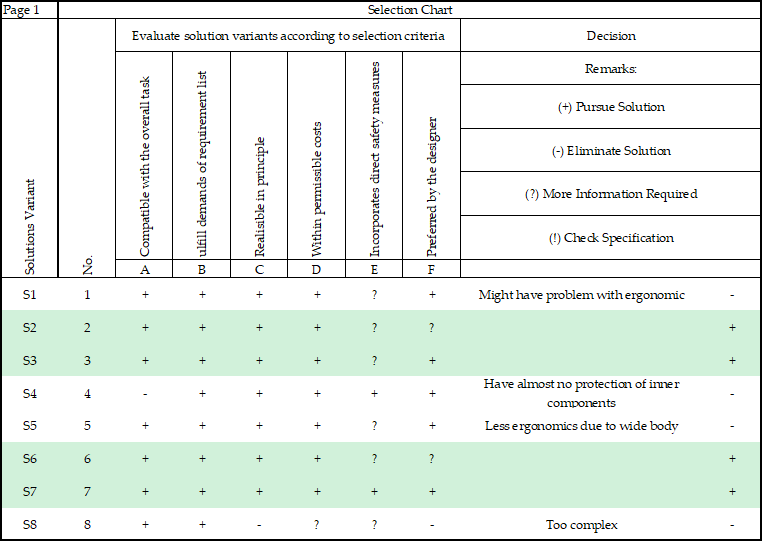
\includegraphics[width=\linewidth]{texs/Part1/chapter3/image/selchart2.png}}
    \caption{Selection Chart for Solution Variants}
    \label{fig:selection-chart-solution-variants}
\end{figure}

The result of the selection chart, as shown in Figure \ref{fig:selection-chart-solution-variants}, indicates that solutions S1, S4, S5, and S8 have been eliminated and will not be considered for the next stage of the design process.

